\section{Progettazione e implementazione dei test unitari}

Per la fase di unit testing sono stati selezionati i seguenti metodi da sottoporre a verifica:

\begin{itemize}
	\item NewDipendenteResponse addDipendente(DipendenteRequest request, String aliasAgenzia)
	\item List<ContattoResponse> aggiungiContatto(ContattoRequest request)
	\item String changePassword(String oldPassword, String newPassword, String confirmPassword)
	\item List<User> utentiInteressati(CriteriDiRicercaUtenti request)
\end{itemize}

\section{addDipendente(DipendenteRequest request, String aliasAgenzia)}

Il metodo \textit{addDipendente}, appartenente alla classe UserService, ha la responsabilità di aggiungere al sistema un nuovo dipendente, che può essere un agente o un manager.

Per questo metodo è stata adottata una strategia di\textbf{ Black Box} Testing, poiché l’obiettivo principale è verificare il comportamento del sistema in base agli stati e ai valori dei parametri in ingresso, senza considerare la logica interna dell’implementazione. In particolare, si è ritenuto fondamentale analizzare le diverse condizioni in cui un dipendente viene correttamente registrato o rifiutato dal sistema.

A tal fine, è stata effettuata una suddivisione dei parametri di input in \textbf{classi di equivalenza}, al fine di individuare i casi validi e non validi da sottoporre a test. Di seguito si riportano le tabelle che documentano tale suddivisione:

\begin{table}[H]
	\centering
	\begin{tabular}{|c|p{4cm}|p{5cm}|c|} 
		\hline
		\textbf{ID Classe} & \textbf{Descrizione} & \textbf{Valore esempio} & \textbf{Validità} \\
		\hline
		DRN1 & L'insieme delle stringe non vuote/lunghezza zero
		& request.nome==Roberto; & Valido \\
		\hline
		DRN2 & L'insieme delle stringhe null/lunghezza zero
		& request.nome=="" & Non Valido \\
		\hline
	\end{tabular}
	\caption{Parametro DipendenteRequest.nome}
	\label{tab:parametriDipendenteRequestNome}
\end{table}

\begin{table}[H]
	\centering
	\begin{tabular}{|c|p{6cm}|p{5cm}|c|} 
		\hline
		\textbf{ID Classe} & \textbf{Descrizione} & \textbf{Valore esempio} & \textbf{Validità} \\
		\hline
		DRC1 & L'insieme delle stringe non vuote/lunghezza zero
		& request.cognome==Morosini; & Valido \\
		\hline
		DRC2 & L'insieme delle stringhe null/lunghezza zero
		& request.cognome==null & Non Valido \\
		\hline
	\end{tabular}
	\caption{Parametro DipendenteRequest.cognome}
	\label{tab:parametriDipendenteRequestCognome}
\end{table}

\begin{table}[H]
	\centering
	\begin{tabular}{|c|p{4cm}|p{5.5cm}|c|} 
		\hline
		\textbf{ID Classe} & \textbf{Descrizione} & \textbf{Valore esempio} & \textbf{Validità} \\
		\hline
		DRR1 & Stringa di valore "AGENT"
		& request.ruolo=="AGENT"; & Valido \\
		\hline
		DRR2 & Stringa di valore "MANAGER"
		& request.ruolo=="MANAGER" & Valido \\
		\hline
		DRR3 & tutti i valori non corrispodenti ad AGENT oppure a MANAGER
		& request.ruolo=="ADMIN" & Non Valido \\
		\hline
		DRR4 & stringa null/lunghezza zero
		& request.ruolo=="" & Non Valido \\
		\hline
	\end{tabular}
	\caption{Parametro DipendenteRequest.ruolo}
	\label{tab:parametriDipendenteRequestRuolo}
\end{table}

\begin{table}[H]
	\centering
	\begin{tabular}{|c|p{4cm}|p{5.5cm}|c|} 
		\hline
		\textbf{ID Classe} & \textbf{Descrizione} & \textbf{Valore esempio} & \textbf{Validità} \\
		\hline
		AA1 & L'insieme delle stringhe non null e non vuoti & aliasAgenzia==RobyImmobili & Valida \\
		\hline
		AA2 & La stringa è null oppure è vuota & aliasAgenzia==null & Non valido \\
		\hline
	\end{tabular}
	\caption{Parametro aliasAgenzia}
	\label{tab:parametriAliasAgenzia}
\end{table}

\vspace{1cm}

Per quanto riguarda la strategia di combinazione dei valori, è stato scelto l’approccio \textbf{R-WECT (Reduced Weak Equivalence Class Testing)}. Questa tecnica è considerata particolarmente robusta perché garantisce:

\begin{itemize}
	\item il test di tutte le classi non valide, ognuna combinata con valori validi per gli altri parametri;
	\item il test di tutte le classi valide per ciascun parametro.
\end{itemize}

Infine, vengono riportati sia il codice sorgente dei test implementati sia l’evidenza del loro esito positivo, a conferma della correttezza delle funzionalità verificate

% Definizione dei colori
\definecolor{bgcolor}{RGB}{245,245,245}    % Sfondo chiaro
\definecolor{keywordcolor}{RGB}{0,0,180}  % Blu per le parole chiave
\definecolor{commentcolor}{RGB}{0,128,0}  % Verde per i commenti
\definecolor{stringcolor}{RGB}{163,21,21} % Rosso per le stringhe

% Configurazione listings
\lstset{
	language=Java,                % Linguaggio di esempio
	backgroundcolor=\color{bgcolor}, % Colore di sfondo
	basicstyle=\ttfamily\small,     % Font e dimensione
	keywordstyle=\color{keywordcolor}\bfseries,
	commentstyle=\color{commentcolor}\itshape,
	stringstyle=\color{stringcolor},
	numbers=left,                   % Numeri a sinistra
	numberstyle=\tiny\color{gray},  % Stile dei numeri
	stepnumber=1,                   % Numeri in ogni riga
	numbersep=5pt,                  % Distanza dai numeri
	frame=single,                   % Cornice intorno al codice
	rulecolor=\color{gray},         % Colore della cornice
	tabsize=4,                       % Tab = 4 spazi
	showstringspaces=false,
	breaklines=true,                  % A capo automatico se troppo lungo
	literate=
		{à}{{\`a}}1
		{è}{{\`e}}1
		{é}{{\'e}}1
		{ì}{{\`i}}1
		{ò}{{\`o}}1
		{ù}{{\`u}}1
}


\begin{lstlisting}
/**
* Test che copre le classi valide: DRN1 (Valida); DRC1 (Valida); DRR1(Valida); AA1(Valida);
*/
@Test
void addDipedenteTestAddAgente(){
	
	DipendenteRequest dipendente = new DipendenteRequest("Roberto", "Spena", "AGENT");
	String dominioAgenzia = "RobyImmobili";
	
	when(userRepository.countByEmail("roberto.spena@robyimmobili.dietiestate.com")).thenReturn(0);
	
	Authority fakeAuthority = new Authority();
	fakeAuthority.setAuthorityName(AuthorityName.AGENT);
	when(authorityRepository.findByAuthorityName(AuthorityName.AGENT)).thenReturn(Optional.of(fakeAuthority));
	
	User fakeUser = new User();
	fakeUser.setId(1); //id fittizio
	DatiImpiegato fakeDati = new DatiImpiegato();
	when(userRepository.save(Mockito.any(User.class))).thenReturn(fakeUser);
	when(datiImpiegatoRepository.save(Mockito.any(DatiImpiegato.class))).thenReturn(fakeDati);
	
	NewDipendeteResponse response = userService.addDipendete(dipendente,dominioAgenzia);
	
	//Controllo email generata
	String emailPrevista = "roberto.spena@robyimmobili.dietiestate.com";
	assertEquals(emailPrevista, response.getUser().getEmail(), "Email non generata correttamente");
	
	//Controllo password generata
	String password = response.getPassword();
	assertEquals(12, password.length(), "La password deve essere lunga 12 caratteri");
	assertTrue(
	password.matches(".*[a-zA-Z].*"),
	"La stringa deve contenere almeno una lettera"
	);
	assertTrue(
	password.matches(".*[!@#$%^&*()\\\\-_=+\\\\[\\\\]{}|;:,.<>?].*"),
	"La stringa deve contenere almeno un carattere speciale"
	);
	assertTrue(
	password.matches(".*[0-9].*"),
	"La stringa deve contenere almeno una cifra"
	);
	
	//Controllo nomeVisualizzato
	String nomeVisualizzato = response.getUser().getNomeVisualizzato();
	String nomeVisualizzatoPrevisto = "Agente Roberto S.";
	assertEquals(nomeVisualizzato, nomeVisualizzatoPrevisto);
	
	//Controllo foto profilo
	String fotoProfilo = response.getUser().getUrlFotoProfilo();
	assertTrue(fotoProfilo.matches("^https://dummyimage.com/.*"), "Url foto profilo non valido");
}
\end{lstlisting}

\begin{lstlisting}
	/**
	*  Test che copre le classi valide: DRN1 (Valida); DRC1 (Valida); DRR2(Valida); AA1(Valida);
	*/
	@Test
	void addDipedenteTestAddManager(){
		
		DipendenteRequest dipendente = new DipendenteRequest("Raimondo", "Morosini", "MANAGER");
		String dominioAgenzia = "RaimondoImmobili";
		
		when(userRepository.countByEmail("raimondo.morosini@raimondoimmobili.dietiestate.com")).thenReturn(0);
		
		Authority fakeAuthority = new Authority();
		fakeAuthority.setAuthorityName(AuthorityName.MANAGER);
		when(authorityRepository.findByAuthorityName(AuthorityName.MANAGER)).thenReturn(Optional.of(fakeAuthority));
		
		User fakeUser = new User();
		fakeUser.setId(1); //id fittizio
		DatiImpiegato fakeDati = new DatiImpiegato();
		when(userRepository.save(Mockito.any(User.class))).thenReturn(fakeUser);
		when(datiImpiegatoRepository.save(Mockito.any(DatiImpiegato.class))).thenReturn(fakeDati);
		
		NewDipendeteResponse response = userService.addDipendete(dipendente,dominioAgenzia);
		
		//Controllo email generata
		String emailPrevista = "raimondo.morosini@raimondoimmobili.dietiestate.com";
		assertEquals(emailPrevista, response.getUser().getEmail(), "Email non generata correttamente");
		
		//Controllo password generata
		String password = response.getPassword();
		assertEquals(12, password.length(), "La password deve essere lunga 12 caratteri");
		assertTrue(
		password.matches(".*[a-zA-Z].*"),
		"La stringa deve contenere almeno una lettera"
		);
		assertTrue(
		password.matches(".*[!@#$%^&*()\\\\-_=+\\\\[\\\\]{}|;:,.<>?].*"),
		"La stringa deve contenere almeno un carattere speciale"
		);
		assertTrue(
		password.matches(".*[0-9].*"),
		"La stringa deve contenere almeno una cifra"
		);
		
		//Controllo nomeVisualizzato
		String nomeVisualizzato = response.getUser().getNomeVisualizzato();
		String nomeVisualizzatoPrevisto = "Manager Raimondo M.";
		assertEquals(nomeVisualizzato, nomeVisualizzatoPrevisto);
		
		//Controllo foto profilo
		String fotoProfilo = response.getUser().getUrlFotoProfilo();
		assertTrue(fotoProfilo.matches("^https://dummyimage.com/.*"), "Url foto profilo non valido");
	}
\end{lstlisting}

\begin{lstlisting}
	/**
	* Test per coprire la classe nome non valida: DRN1 (Non Valida); DRC1 (Valida); DRR2(Valida); AA1(Valida);
	*/
	@Test
	void addDipedenteTestNomeNonValido(){
		
		DipendenteRequest dipendente = new DipendenteRequest(null, "Sepe", "MANAGER");
		String dominioAgenzia = null;
		
		Exception ex = assertThrows(IllegalArgumentException.class, () -> userService.addDipendete(dipendente,dominioAgenzia));
		
		assertTrue(ex.getMessage().contains("Il parametro nome è vuoto."));
	}
\end{lstlisting}

\begin{lstlisting}
	 /**
	* Test per coprire la classe cognome non valida: DRN1 (Valida); DRC1 (Non Valida); DRR2(Valida); AA1(Valida);
	*/
	@Test
	void addDipedenteTestCognomeNonValido(){
		
		DipendenteRequest dipendente = new DipendenteRequest("Lorenzo", "", "MANAGER");
		String dominioAgenzia = "LorenzoImmobili";
		
		Exception ex = assertThrows(IllegalArgumentException.class, () -> userService.addDipendete(dipendente,dominioAgenzia));
		
		assertTrue(ex.getMessage().contains("Il parametro cognome è vuoto."));
	}
\end{lstlisting}

\begin{lstlisting}
	/**
	*  Test per coprire la classe ruolo non valida: DRN1 (Valida); DRC1 (Valida); DRR2(Non Valida); AA1(Valida);
	*/
	@Test
	void addDipedenteTestRuoloNonValido(){
		
		DipendenteRequest dipendente = new DipendenteRequest("", "Sepe", "ADMIN");
		String dominioAgenzia = "LorenzoImmobili";
		
		Exception ex = assertThrows(IllegalArgumentException.class, () -> userService.addDipendete(dipendente,dominioAgenzia));
		
		assertTrue(ex.getMessage().contains("Ruolo non valido:"));
	}
\end{lstlisting}

\begin{lstlisting}
	/**
	*  Test per coprire la classe ruolo non esistente: DRN1 (Valida); DRC1 (Valida); DRR4(Non Valida); AA1(Valida);
	*/
	@Test
	void addDipedenteTestRuoloInesistente(){
		
		DipendenteRequest dipendente = new DipendenteRequest("", "Sepe", "");
		String dominioAgenzia = "LorenzoImmobili";
		
		Exception ex = assertThrows(IllegalArgumentException.class, () -> userService.addDipendete(dipendente,dominioAgenzia));
		
		assertTrue(ex.getMessage().contains("Ruolo inesistente"));
	}
\end{lstlisting}

\begin{lstlisting}
	 /**
	* Test per coprire la classe aliasAgeniza non valida: DRN1 (Valida); DRC1 (Valida); DRR2(Valida); AA1(Non Valida);
	*/
	@Test
	void addDipedenteTestDominioAgenziaNonValido(){
		
		DipendenteRequest dipendente = new DipendenteRequest("Lorenzo", "Sepe", "MANAGER");
		String dominioAgenzia = null;
		
		Exception ex = assertThrows(IllegalArgumentException.class, () -> userService.addDipendete(dipendente,dominioAgenzia));
		
		assertTrue(ex.getMessage().contains("Il parametro aliasAgenzia è vuoto."));
	}
\end{lstlisting}

\begin{figure}[H]
	\centering
	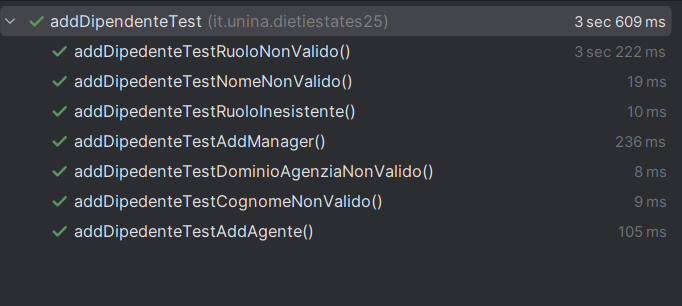
\includegraphics[width=0.7\linewidth]{Immagini/unit test/esitiTestAddDipendente.png}
	\caption[Esito test]{Screen che riporta l'esito positivo dei test}
\end{figure}


\section{utentiInteressati(CriteriDiRicercaUtenti request)}

Il metodo \colorbox{lightgray}{utentiInteressati}, appartenente alla classe \colorbox{lightgray}{RicercaAnnunciEffettuatiService}, ha la responsabilità di individuare tutti gli utenti potenzialmente interessati in base alle ricerche che essi hanno precedentemente effettuato.
Questo metodo viene invocato quando il sistema deve inviare una notifica e necessita di filtrare i destinatari realmente pertinenti. Il parametro di ingresso, \colorbox{lightgray}{CriteriDiRicercaUtenti}, contiene i campi relativi alle caratteristiche di un immobile. Se i criteri passati al metodo corrispondono a quelli di una ricerca salvata da un utente nel sistema, tale utente viene incluso nella lista dei destinatari risultanti.
\newline
Per la progettazione dei test unitari è stata adottata una \textbf{strategia di tipo black-box}, analogamente a quanto fatto per il metodo \colorbox{lightgray} {addDipendente}. Tuttavia, la motivazione alla base di questa scelta è differente: mentre nel test di \colorbox{lightgray}{addDipendente} l’obiettivo è verificare che il dipendente aggiunto possieda i valori corretti in funzione della richiesta di input, nel caso di \colorbox{lightgray}{utentiInteressati} l’attenzione è rivolta al comportamento del metodo rispetto ai criteri di ricerca forniti.
In particolare, si verifica che i valori non validi (ad esempio campi vuoti o non significativi) presenti nel parametro \colorbox{lightgray}{CriteriDiRicercaUtenti} vengano opportunamente impostati a \colorbox{lightgray}{null}, in modo da escluderli dal processo di matching con le ricerche salvate. Questo controllo è fondamentale per garantire che il sistema notifichi esclusivamente gli utenti realmente interessati.

Di seguito si riportano le tabelle che documentano tale suddivisione:

\begin{table}[H]
	\centering
	\begin{tabular}{|c|p{4cm}|p{6cm}|c|} 
		\hline
		\textbf{ID Classe} & \textbf{Descrizione} & \textbf{Valore esempio} & \textbf{Validità} \\
		\hline
		A1 & L'insieme delle stringe che corrispondo a una località italiana
		& request.areaDiInteresse==Napoli & Valido \\
		\hline
		A2 & L'insieme delle stringhe null/lunghezza zero
		& request.areaDiInteresse==null & Valido \\
		\hline
		A3 & L'insieme delle stringhe che non corrispondono a una località italiana
		& request.areaDiInteresse==città inesistente & Valido \\
		\hline
	\end{tabular}
	\caption{Parametro request.areaDiInteresse}
	\label{tab:parametriRequestAreaDiInteresse}
\end{table}

\begin{table}[H]
	\centering
	\begin{tabular}{|c|p{6cm}|p{6.2cm}|c|} 
		\hline
		\textbf{ID Classe} & \textbf{Descrizione} & \textbf{Valore esempio} & \textbf{Validità} \\
		\hline
		C1 & Un valore dell'enumerazione (AFFITTO,VENDITA)
		& request.tipoDiContrattoDiInteresse == AFFITTO; & Valido \\
		\hline
		C2 & valore null
		& request.tipoDiContrattoDiInteresse == null & Valido \\
		\hline
	\end{tabular}
	\caption{Parametro request.tipoDiContrattoDiInteresse}
	\label{tab:parametriRequestTipoDiContrattoDiInteresse}
\end{table}

\begin{table}[H]
	\centering
	\begin{tabular}{|c|p{6cm}|p{6.2cm}|c|} 
		\hline
		\textbf{ID Classe} & \textbf{Descrizione} & \textbf{Valore esempio} & \textbf{Validità} \\
		\hline
		I1 & Un valore dell'enumerazione
		& request.tipoDiImmobileDiInteresse == APPARTAMENTO; & Valido \\
		\hline
		I2 & valore null
		& request.tipoDiContrattoDiInteresse == null & Valido \\
		\hline
	\end{tabular}
	\caption{Parametro request.tipoDiImmobileDiInteresse}
	\label{tab:parametriRequestTipoDiImmobileDiInteresse}
\end{table}

\begin{table}[H]
	\centering
	\begin{tabular}{|c|p{4cm}|p{5.5cm}|c|} 
		\hline
		\textbf{ID Classe} & \textbf{Descrizione} & \textbf{Valore esempio} & \textbf{Validità} \\
		\hline
		BMI1 & Qualsiasi numero positivo
		& request.budgetMin==100 & Valido \\
		\hline
		BMI2 & qualsiasi numero negativo
		& request.budgetMin==-100 & Valido \\
		\hline
		BMI3 & valore null
		& request.budgetMin==null & Valido \\
		\hline
	\end{tabular}
	\caption{Parametro request.budgetMin}
	\label{tab:parametriRequestBudgetMin}
\end{table}

\begin{table}[H]
	\centering
	\begin{tabular}{|c|p{4cm}|p{5.5cm}|c|} 
		\hline
		\textbf{ID Classe} & \textbf{Descrizione} & \textbf{Valore esempio} & \textbf{Validità} \\
		\hline
		BMA1 & Qualsiasi numero positivo
		& request.budgetMan==600 & Valido \\
		\hline
		BMA2 & qualsiasi numero negativo
		& request.budgetMax==-600 & Valido \\
		\hline
		BMA3 & valore null
		& request.budgetMin==null & Valido \\
		\hline
	\end{tabular}
	\caption{Parametro request.budgetMax}
	\label{tab:parametriRequestBudgetMax}
\end{table}

\begin{table}[H]
	\centering
	\begin{tabular}{|c|p{4cm}|p{5.5cm}|c|} 
		\hline
		\textbf{ID Classe} & \textbf{Descrizione} & \textbf{Valore esempio} & \textbf{Validità} \\
		\hline
		IG1 & Qualsiasi intero positivo & request.intervalloGiorni==10 & Valida \\
		\hline
		II2 & intero negativo & request.intervalloGiorni==-1 & Valido \\
		\hline
		II3 & Valore null & request.intervalloGiorni==null & Valido \\
		\hline
	\end{tabular}
	\caption{Parametro request.intervalloGiorniStoricoRicerche}
	\label{tab:parametriRequestIntervalloGiorniStoricoRicerche}
\end{table}

\vspace{1cm}

% Definizione dei colori
\definecolor{bgcolor}{RGB}{245,245,245}    % Sfondo chiaro
\definecolor{keywordcolor}{RGB}{0,0,180}  % Blu per le parole chiave
\definecolor{commentcolor}{RGB}{0,128,0}  % Verde per i commenti
\definecolor{stringcolor}{RGB}{163,21,21} % Rosso per le stringhe


% Configurazione listings
\lstset{
	language=Java,                % Linguaggio di esempio
	backgroundcolor=\color{bgcolor}, % Colore di sfondo
	basicstyle=\ttfamily\small,     % Font e dimensione
	keywordstyle=\color{keywordcolor}\bfseries,
	commentstyle=\color{commentcolor}\itshape,
	stringstyle=\color{stringcolor},
	numbers=left,                   % Numeri a sinistra
	numberstyle=\tiny\color{gray},  % Stile dei numeri
	stepnumber=1,                   % Numeri in ogni riga
	numbersep=5pt,                  % Distanza dai numeri
	frame=single,                   % Cornice intorno al codice
	rulecolor=\color{gray},         % Colore della cornice
	tabsize=4,                       % Tab = 4 spazi
	showstringspaces=false,
	breaklines=true,                  % A capo automatico se troppo lungo
	literate=
		{à}{{\`a}}1
		{è}{{\`e}}1
		{é}{{\'e}}1
		{ì}{{\`i}}1
		{ò}{{\`o}}1
		{ù}{{\`u}}1
}

Prima di ogni test vengono eseguiti i settaggi di deafult della request in modo che venga modificato solo il campo di interesse i ogni test.
Mentre dopo eseguito ogni test viene verificato che alla repository, che interroga il db ed esegue il processo di corrispondenza, vengono passati i parametri che sono impostati nella request. Di seguito mostriamo il codice di tale settaggio.

\begin{lstlisting}
@BeforeEach 
void setup() {
	ricercaAnnunciEffettuataService = new RicercaAnnunciEffettuataService(mockRicercaAnnunciEffettuataRepository,MockUserRepository,new HashSet<String>());
	request = CriteriDiRicercaUtenti.builder()
	.intervalloGiorniStoricoRicerca(10)
	.tipoDiContrattoDiInteresse(TipoContratto.AFFITTO)
	.tipologiaDiImmobileDiInteresse(TipologiaImmobile.APPARTAMENTO)
	.budgetMin(BigDecimal.valueOf(100))
	.budgetMax(BigDecimal.valueOf(600))
	.areaDiInteresse("Napoli")
	.build();
}


@AfterEach 
void verifyRepositorySave() {
	verify(mockRicercaAnnunciEffettuataRepository).trovaUtentiPerCriteri(
	eq(request.getBudgetMin()),
	eq(request.getBudgetMax()),
	eq(request.getAreaDiInteresse()),
	eq(request.getTipoDiContrattoDiInteresse()),
	eq(request.getTipologiaDiImmobileDiInteresse()),
	any(LocalDateTime.class)  // qualsiasi valore va bene
	);
	
	
}
\end{lstlisting}

La suddivisione in classi di equivalenza dei parametri di questo metodo non presenta classi non valide, poiché, come spiegato, i campi con valori non validi vengono impostati a un valore specifico, come ad esempio \colorbox{lightgray}{null}.
La strategia utilizzata per la combinazione dei test consiste nel verificare tutte le classi valide con parametri validi e, successivamente, nell’eseguire un test per ciascun caso in cui un solo campo assume un valore non valido mentre tutti gli altri rimangono validi.


\begin{lstlisting}
	 /**
	* test con area di interesse Italia non deve modificare nulla tranne l'area di interesse che deve settarla a null
	*/
	@Test
	void areaDiInteresseItaliaShouldSetNullAreaDiInteresse() {
		request.setAreaDiInteresse("Italia");
		ricercaAnnunciEffettuataService.utentiInteressati(request);
		assertTrue(request.getAreaDiInteresse()==null);
	}
\end{lstlisting}

\begin{lstlisting}
	/**
	* test che controlla che se il budget max è minore del budget min, li scambia
	*/
	@Test
	void budgetMaxLessThanBudgetMinShouldSwapThem() {
		request.setBudgetMin(BigDecimal.valueOf(600));
		request.setBudgetMax(BigDecimal.valueOf(100));
		ricercaAnnunciEffettuataService.utentiInteressati(request);
		assertTrue(request.getBudgetMin().equals(BigDecimal.valueOf(100)));
		assertTrue(request.getBudgetMax().equals(BigDecimal.valueOf(600)));
	}
\end{lstlisting}

\begin{lstlisting}
	/**
	* Test che controlla che se la città non esiste, imposta a null il campo area di interesse della request
	*/
	@Test
	void invalidCityShouldSetNullAreaDiInteresse() {
		request.setAreaDiInteresse("Città Inesistente");
		ricercaAnnunciEffettuataService.utentiInteressati(request);
		assertTrue(request.getAreaDiInteresse()==null);
	}
\end{lstlisting}

\begin{lstlisting}
	/**
	* test che controlla che se budget min è negativo, lo imposta a null
	*/
	@Test
	void negativeBudgetMinShouldSetNullBudgetMin() {
		request.setBudgetMin(BigDecimal.valueOf(-100));
		ricercaAnnunciEffettuataService.utentiInteressati(request);
		
		assertTrue(request.getBudgetMin()==null);
	}
\end{lstlisting}

\begin{lstlisting}
	/**
	* test che controlla che se budget max è negativo, lo imposta a null
	*/
	@Test
	void negativeBudgetMaxShouldSetNullBudgetMax() {
		request.setBudgetMax(BigDecimal.valueOf(-100));
		ricercaAnnunciEffettuataService.utentiInteressati(request);
		assertTrue(request.getBudgetMax()==null);
	}
\end{lstlisting}

\begin{lstlisting}
	/**
	* test che controlla se l' intervallo di giorni è negativo, lo imposta setta a 7
	*/
	@Test
	void deltaDaysLessThanZeroShouldSet7() {
		request.setIntervalloGiorniStoricoRicerca(0);
		ricercaAnnunciEffettuataService.utentiInteressati(request);
		assertTrue(request.getIntervalloGiorniStoricoRicerca()==7);
		
	}
\end{lstlisting}


\begin{figure}[H]
	\centering
	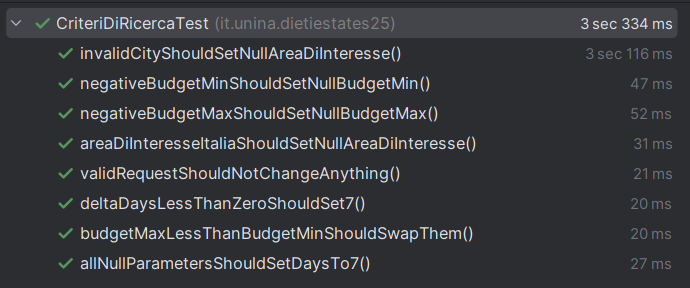
\includegraphics[width=0.7\linewidth]{Immagini/unit test/esitiTestUtentiInteressati.png}
	\caption[Esito test 2]{Screen che riporta l'esito positivo dei test}
\end{figure}


\subsection{aggiungiContatto(ContattoRequest request)}

Il metodo  \colorbox{lightgray}{aggiungiContatto()}, appartenente alla classe DatiImpiegatoService, è responsabile dell’aggiunta di un contatto di riferimento per un agente immobiliare.
Per la verifica del suo corretto funzionamento è stata adottata una \textbf{strategia di testing white-box}, poiché il metodo presenta diversi flussi di controllo interni. Questa scelta consente di verificare che, a fronte di specifici input, il metodo segua il percorso logico previsto.
\\
In particolare, il metodo deve distinguere tra due casi:
\begin{enumerate}
	\item \textbf{Il contatto esiste già}: in questo scenario, il metodo aggiorna il valore del contatto esistente.
	\item \textbf{Il contatto non esiste}: in tal caso, viene aggiunto un nuovo elemento alla lista dei contatti.
\end{enumerate}
Di seguito è riportato il \textbf{grafo del flusso di controllo (GFC)}, utilizzato per rappresentare visivamente le diverse diramazioni logiche del metodo.

\begin{figure}[H]
	\centering
	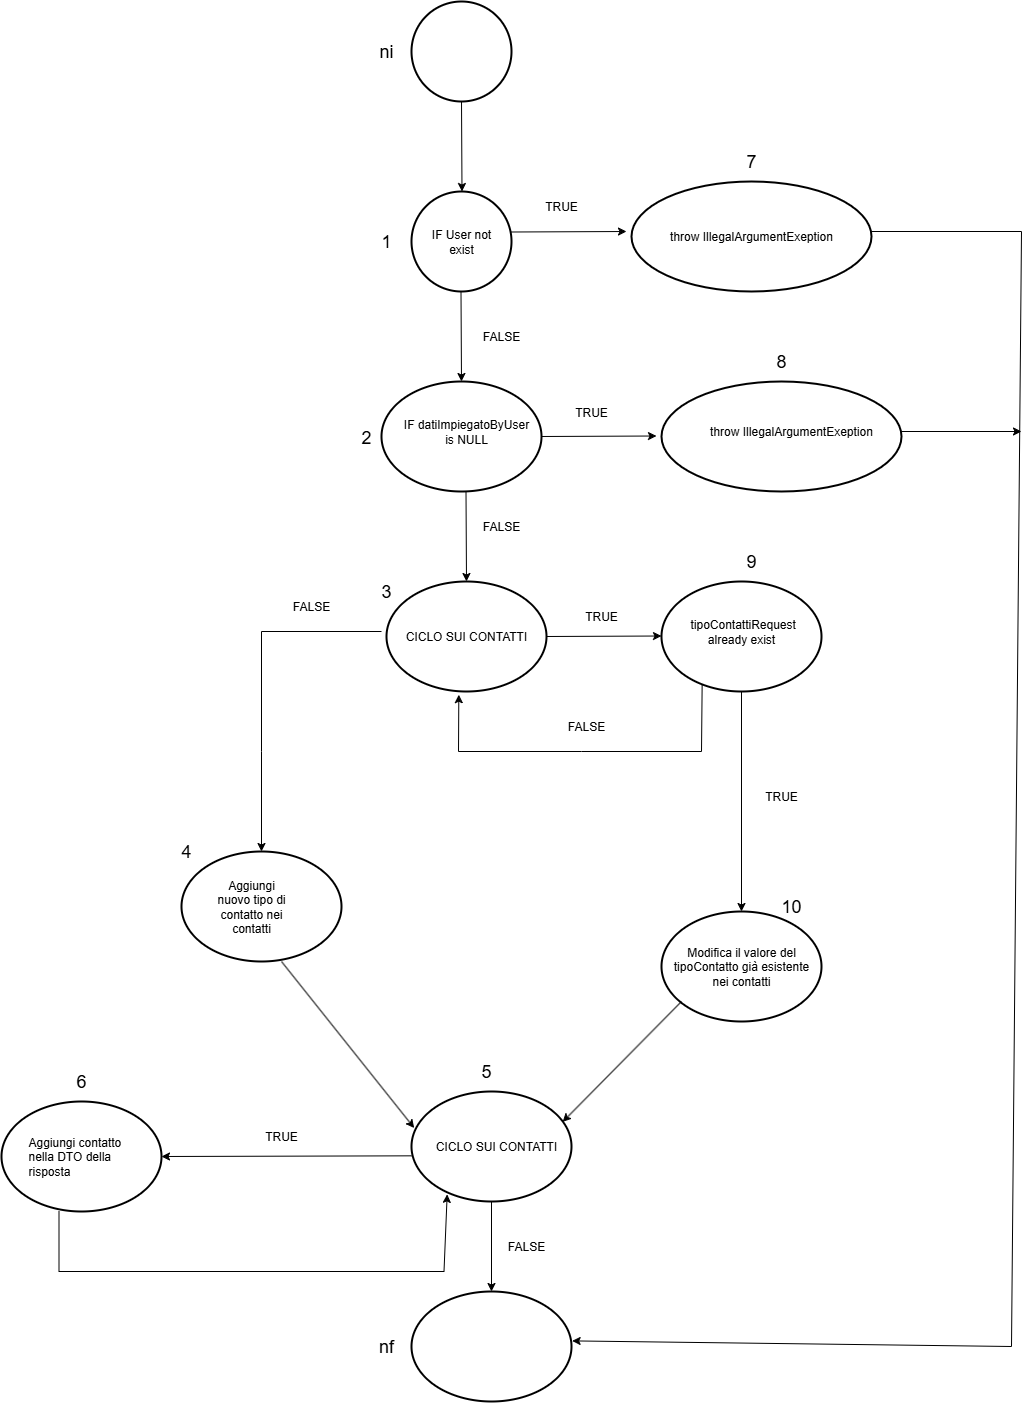
\includegraphics[width=0.7\linewidth]{Immagini/unit test/GrafoAggiungiUnContatto.png}
	\caption[GFC aggiungiContatto]{GFC del metodo aggiungiContatto(ContattoRequest request)}
\end{figure}

% Configurazione listings
\lstset{
	language=Java,                % Linguaggio di esempio
	backgroundcolor=\color{bgcolor}, % Colore di sfondo
	basicstyle=\ttfamily\small,     % Font e dimensione
	keywordstyle=\color{keywordcolor}\bfseries,
	commentstyle=\color{commentcolor}\itshape,
	stringstyle=\color{stringcolor},
	numbers=left,                   % Numeri a sinistra
	numberstyle=\tiny\color{gray},  % Stile dei numeri
	stepnumber=1,                   % Numeri in ogni riga
	numbersep=5pt,                  % Distanza dai numeri
	frame=single,                   % Cornice intorno al codice
	rulecolor=\color{gray},         % Colore della cornice
	tabsize=4,                       % Tab = 4 spazi
	showstringspaces=false,
	breaklines=true,                  % A capo automatico se troppo lungo
	literate=
	{à}{{\`a}}1
	{è}{{\`e}}1
	{é}{{\'e}}1
	{ì}{{\`i}}1
	{ò}{{\`o}}1
	{ù}{{\`u}}1
}


I test eseguiti hanno lo scopo di testare tutti i cammini possibili del grafo.

\begin{lstlisting}
	/**
	* Test verifica l'eccezione in caso di UserCurrent non trovato.
	* Copertura 1-7
	*/
	@Test
	void aggiungiContatto_ShouldThrowUnauthorizedException_
		WhenUserContextNotFound(){
		
			mocked.when(UserContex::getUserCurrent).thenReturn(null);
			
			assertThrows(it.unina.dietiestates25.exception.UnauthorizedException.class, () ->
			datiImpiegatoService.aggiungiContatto(request));
	}
\end{lstlisting}

\begin{lstlisting}
		/**
		* verifica che venga lanciata una ResourceNotFoundException quando l'utente non viene trovato nel database.
		* Copertura cammino 1-2-8
		*/
		@Test
		void aggiungiContatto_ShouldThrowResourceNotFoundException_
			WhenUserNotFoundInDB(){
			
				User mockUser = new User();
				
				mocked.when(UserContex::getUserCurrent).thenReturn(mockUser);
				when(datiImpiegatoRepository.findDatiImpiegatoByUser(mockUser)).thenReturn(Optional.empty());
				
				assertThrows(it.unina.dietiestates25.exception.ResourceNotFoundException.class, () ->
				datiImpiegatoService.aggiungiContatto(request));
			
		}
\end{lstlisting}

\begin{lstlisting}
	 /**
	* Verifica che aggiunge un nuovo contatto tra i contatti già esistenti dell'agente
	* Copertura cammino 1-2-3-4-5-6-5
	*/
	@Test
	void aggiungiContatto_
	ShouldAddNewContactWithoutExistingContacts(){
		
			request.setTipo("Cellulare");
			request.setValore("338469123");
			
			List<ContattoResponse> response = datiImpiegatoService.aggiungiContatto(request);
			
			//Controlli sul nuovo stato dei contatti esistenti dell'agente
			assertTrue(contattiEsistenti.size() == 1);
			assertTrue(contattiEsistenti.get(0).getTipo().equals("Cellulare"));
			assertTrue(contattiEsistenti.get(0).getValore().equals("338469123"));
			
			//Controlli sulla DTO in risposta
			assertTrue(response.size() == 1);
			
			assertTrue(response.get(0).getTipo().equals("Cellulare"));
			assertTrue(response.get(0).getValore().equals("338469123"));
	}
\end{lstlisting}

\begin{lstlisting}
	/**
	* Verica che aggiunge un nuovo contatto (come sopra ma con almeno un iterazione tra i contati esistenti)
	*Copertura cammino 1-2-3-9-3-4-5-6-5-6-5
	*/
	@Test
	void aggiungiContatto_
	ShouldAddNewConcatWithExistingContacts(){
		
			Contatto contatto = Contatto.builder()
			.tipo("Cellulare")
			.valore("3338469123")
			.build();
			
			contattiEsistenti.add(contatto);
			
			request.setTipo("Email");
			request.setValore("roby@gmail.com");
			
			List<ContattoResponse> response = datiImpiegatoService.aggiungiContatto(request);
			
			//Controlli sul nuovo stato dei contatti esistenti dell'agente
			assertTrue(contattiEsistenti.size() == 2);
			
			assertTrue(contattiEsistenti.get(0).getTipo().equals("Cellulare"));
			assertTrue(contattiEsistenti.get(0).getValore().equals("3338469123"));
			
			assertTrue(contattiEsistenti.get(1).getTipo().equals("Email"));
			assertTrue(contattiEsistenti.get(1).getValore().equals("roby@gmail.com"));
			
			//Controlli sulla DTO in risposta
			assertTrue(response.size() == 2);
			
			assertTrue(response.get(0).getTipo().equals("Cellulare"));
			assertTrue(response.get(0).getValore().equals("3338469123"));
			
			assertTrue(response.get(1).getTipo().equals("Email"));
			assertTrue(response.get(1).getValore().equals("roby@gmail.com"));
	}
\end{lstlisting}

\begin{lstlisting}
	/**
	* verifica che si accorge che il contatto è un tipo già esistente e quindi deve modificarne il valore non aggiungere uno nuovo.
	* Copertura cammino 1-2-3-9-3-9-10-5-6-5-6-5
	*/
	@Test
	void aggiungiContatto_ShouldModifyExistingContact(){
		
		Contatto contatto1 = Contatto.builder()
		.tipo("Cellulare")
		.valore("3338469123")
		.build();
		
		Contatto contatto2 = Contatto.builder()
		.valore("roby@gmail.com")
		.tipo("Email")
		.build();
		
		contattiEsistenti.add(contatto1);
		contattiEsistenti.add(contatto2);
		
		request.setTipo("Email");
		request.setValore("raimondo@gmail.com");
		
		List<ContattoResponse> response = datiImpiegatoService.aggiungiContatto(request);
		
		//Controlli sul nuovo stato dei contatti esistenti dell'agente
		assertTrue(contattiEsistenti.size() == 2);
		
		assertTrue(contattiEsistenti.get(0).getTipo().equals("Cellulare"));
		assertTrue(contattiEsistenti.get(0).getValore().equals("3338469123"));
		
		assertTrue(contattiEsistenti.get(1).getTipo().equals("Email"));
		assertTrue(contattiEsistenti.get(1).getValore().equals("raimondo@gmail.com"));
		
		//Controlli sulla DTO in risposta
		assertTrue(response.size() == 2);
		
		assertTrue(response.get(0).getTipo().equals("Cellulare"));
		assertTrue(response.get(0).getValore().equals("3338469123"));
		
		assertTrue(response.get(1).getTipo().equals("Email"));
		assertTrue(response.get(1).getValore().equals("raimondo@gmail.com"));
		
	}
\end{lstlisting}

\begin{lstlisting}
	  /**
	* verifica che si accorge di moficare il valore di un contatto invece di aggiungerlo uno nuovo. (Stessa verifica di sopra ma senza iterazione nel ciclo)
	* Copertura cammino 1-2-3-9-10-5-6-5
	*/
	@Test
	void aggiungiContatto_
	ShouldModifyExistingContactWithoutIteration(){
		
			Contatto contatto = Contatto.builder()
			.tipo("Cellulare")
			.valore("3338469123")
			.build();
			
			contattiEsistenti.add(contatto);
			
			request.setTipo("Cellulare");
			request.setValore("31520289137");
			
			List<ContattoResponse> response = datiImpiegatoService.aggiungiContatto(request);
			
			//Controlli sul nuovo stato dei contatti esistenti dell'agente
			assertTrue(contattiEsistenti.size() == 1);
			
			assertTrue(contattiEsistenti.get(0).getTipo().equals("Cellulare"));
			assertTrue(contattiEsistenti.get(0).getValore().equals("31520289137"));
			
			//Controlli sulla DTO in risposta
			assertTrue(response.size() == 1);
			
			assertTrue(response.get(0).getTipo().equals("Cellulare"));
			assertTrue(response.get(0).getValore().equals("31520289137"));
		
	}
\end{lstlisting}

\begin{figure}[H]
	\centering
	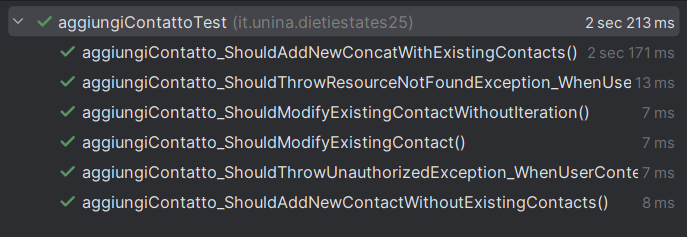
\includegraphics[width=0.7\linewidth]{Immagini/unit test/esitiTestaddContatto.png}
	\caption[Esito test 3]{Screen che riporta l'esito positivo dei test}
\end{figure}


\subsection{changePassword(String oldPassword, String newPassword, String confirmPassword)}

Il metodo \colorbox{lightgray}{changePassword}, appartenente alla classe \colorbox{lightgray}{AuthService}, è responsabile della modifica della password di un utente. Per la sua particolare struttura, si è scelto di adottare una \textbf{strategia di testing white-box}, poiché il metodo è costituito principalmente da \textbf{controlli logici} e di contesto, come la verifica della correttezza della vecchia password e la conformità della nuova password al pattern richiesto.
\\
Di seguito è riportato il \textbf{Grafo del Flusso di Controllo del metodo}, seguito dai \textbf{test case} sviluppati per garantire la copertura di \textbf{tutti i cammini possibili} all’interno del grafo.

\begin{figure}[H]
	\centering
	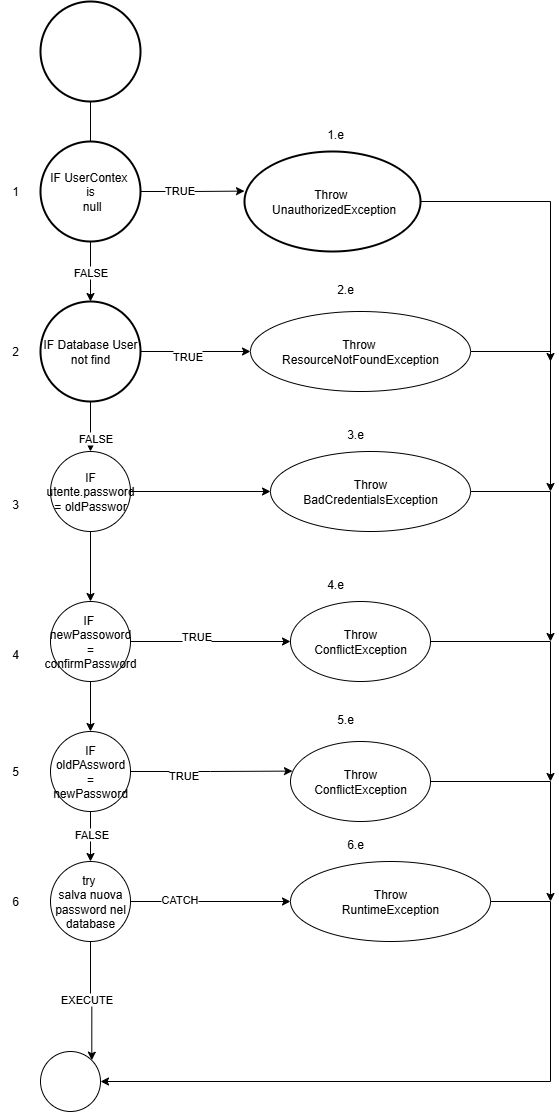
\includegraphics[width=0.7\linewidth]{Immagini/unit test/grafoCambiaPassword.png}
	\caption[GFC changePassword]{GFC del metodo changePassword(String oldPassword, String newPassword, String confirmPassword)}
\end{figure}

% Configurazione listings
\lstset{
	language=Java,                % Linguaggio di esempio
	backgroundcolor=\color{bgcolor}, % Colore di sfondo
	basicstyle=\ttfamily\small,     % Font e dimensione
	keywordstyle=\color{keywordcolor}\bfseries,
	commentstyle=\color{commentcolor}\itshape,
	stringstyle=\color{stringcolor},
	numbers=left,                   % Numeri a sinistra
	numberstyle=\tiny\color{gray},  % Stile dei numeri
	stepnumber=1,                   % Numeri in ogni riga
	numbersep=5pt,                  % Distanza dai numeri
	frame=single,                   % Cornice intorno al codice
	rulecolor=\color{gray},         % Colore della cornice
	tabsize=4,                       % Tab = 4 spazi
	showstringspaces=false,
	breaklines=true,                  % A capo automatico se troppo lungo
	literate=
	{à}{{\`a}}1
	{è}{{\`e}}1
	{é}{{\'e}}1
	{ì}{{\`i}}1
	{ò}{{\`o}}1
	{ù}{{\`u}}1
}


\begin{lstlisting}
	 /**
	*  Questo test copre i nodi da 1 al 6 percorrendo solo il cammino senza errori.
	*/
	@Test
	void changePassword_ShouldSave_WhenValid() {
		User mockUser = new User();
		mockUser.setId(1);
		
		mockUser.setPassword(passwordEncoder.encode("oldPass"));
		
		
		mocked.when(UserContex::getUserCurrent).thenReturn(mockUser);
		
		when(userRepository.findById(1)).thenReturn(Optional.of(mockUser));
		
		String result = authService.changePassword("oldPass", "newPass", "newPass");
		
		verify(userRepository).save(mockUser);
		assertEquals(Msg.PASSWORD_CHANGED, result);
		//assert true when password encorder match new password with mockUser password
		assertTrue(passwordEncoder.matches("newPass", mockUser.getPassword()));
		
	}
\end{lstlisting}

\begin{lstlisting}
	/**
	* Questo test copre il nodo 1 e 1.e
	* * verifica che venga lanciata una UnauthorizedException quando l'utente non viene trovato nel userContex.
	*/
	@Test
	void changePassword_
	ShouldThrowUnauthorizedException_WhenUserContextNotFound() {
		
		mocked.when(UserContex::getUserCurrent).thenReturn(null);
		Exception ex = assertThrows(it.unina.dietiestates25.exception.UnauthorizedException.class, () ->authService.changePassword("oldPass", "newPass", "newPass") );
	}
\end{lstlisting}
	
\begin{lstlisting}
	/**
	* Questo test copre i nodi 1, 2, 2.e
	* * verifica che venga lanciata una ResourceNotFoundException quando l'utente non viene trovato nel database.
	*/
	@Test
	void changePassword_
	ShouldThrowResourceNotFoundException_WhenUserNotFoundInDB() {
		
		User mockUser = new User();
		mockUser.setId(1);
		
		
		mocked.when(UserContex::getUserCurrent).thenReturn(mockUser);
		
		when(userRepository.findById(1)).thenReturn(Optional.empty());
		
		assertThrows(it.unina.dietiestates25.exception.ResourceNotFoundException.class, () ->authService.changePassword("oldPass", "newPass", "newPass") );
		
	}
\end{lstlisting}
	
\begin{lstlisting}
	/**
	* Questo test copre i nodi 1, 2, 3, 3.e
	* * verifica che venga lanciata una BadCredentialsException quando la vecchia password non corrisponde alla password corrente del user.
	*/
	@Test
	void changePassword_
	ShouldThrowBadCredentialsException_WhenOldPasswordNotMatch() {
		User mockUser = new User();
		mockUser.setId(1);
		mockUser.setPassword(passwordEncoder.encode("oldPass"));
		
		mocked.when(UserContex::getUserCurrent).thenReturn(mockUser);
		
		when(userRepository.findById(1)).thenReturn(Optional.of(mockUser));
		
		assertThrows(BadCredentialsException.class, () ->authService.changePassword("wrongOldPass", "newPass", "newPass") );
	}
\end{lstlisting}

\begin{lstlisting}
	/**
	* Questo test copre i nodi 1, 2, 3, 4, 4.e
	* * verifica che venga lanciata una ConflictException quando la nuova password e la password di conferma non corrispondono.
	*/
	@Test
	void changePassword_ShouldThrowConflictException
	_WhenNewPasswordNotMatchConfirmPassword() {
		
		User mockUser = new User();
		mockUser.setId(1);
		mockUser.setPassword(passwordEncoder.encode("oldPass"));
		
		mocked.when(UserContex::getUserCurrent).thenReturn(mockUser);
		
		when(userRepository.findById(1)).thenReturn(Optional.of(mockUser));
		
		assertThrows(it.unina.dietiestates25.exception.ConflictException.class, () ->authService.changePassword("oldPass", "newPass", "differentNewPass") );
	}
\end{lstlisting}

\begin{lstlisting}
	 /**
	* Questo test copre i nodi 1, 2, 3, 4, 5, 5.e
	* * verifica che venga lanciata una ConflictException quando la nuova password è uguale alla password attuale.
	*/
	@Test
	void changePassword_ShouldThrowConflictException
	_WhenNewPasswordIsSameAsOldPassword() {
		User mockUser = new User();
		mockUser.setId(1);
		mockUser.setPassword(passwordEncoder.encode("oldPass"));
		
		mocked.when(UserContex::getUserCurrent).thenReturn(mockUser);
		
		when(userRepository.findById(1)).thenReturn(Optional.of(mockUser));
		
		assertThrows(it.unina.dietiestates25.exception.ConflictException.class, () ->authService.changePassword("oldPass", "oldPass", "oldPass") );
	}
\end{lstlisting}

\begin{lstlisting}
	/**
	* Questo test copre i nodi 1, 2, 3, 4, 5, 6, 6.e
	* * verifica che venga lanciata una RuntimeException quando si verifica un errore durante il salvataggio della nuova password.
	*/
	@Test
	void changePassword_ShouldThrowRuntimeException_WhenErrorOnSave() {
		User mockUser = new User();
		
		mockUser.setId(1);
		mockUser.setPassword(passwordEncoder.encode("oldPass"));
		
		
		mocked.when(UserContex::getUserCurrent).thenReturn(mockUser);
		
		when(userRepository.findById(1)).thenReturn(Optional.of(mockUser));
		//simula un errore durante il salvataggio
		when(userRepository.save(mockUser)).thenThrow(new RuntimeException());
		
		assertThrows(RuntimeException.class, () ->authService.changePassword("oldPass", "newPass", "newPass") );
	}
\end{lstlisting}

\begin{figure}[H]
	\centering
	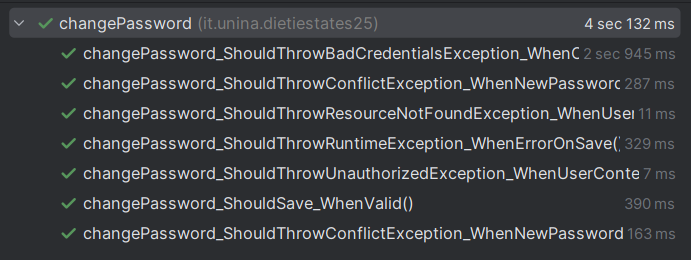
\includegraphics[width=0.7\linewidth]{Immagini/unit test/esitiTestChangePassword.png}
	\caption[Esito test 4]{Screen che riporta l'esito positivo dei test}
\end{figure}
